\documentclass[tikz,border=3mm]{standalone}
\usepackage[siunitx]{circuitikz}
\usetikzlibrary{calc,positioning,arrows.meta}

\begin{document}

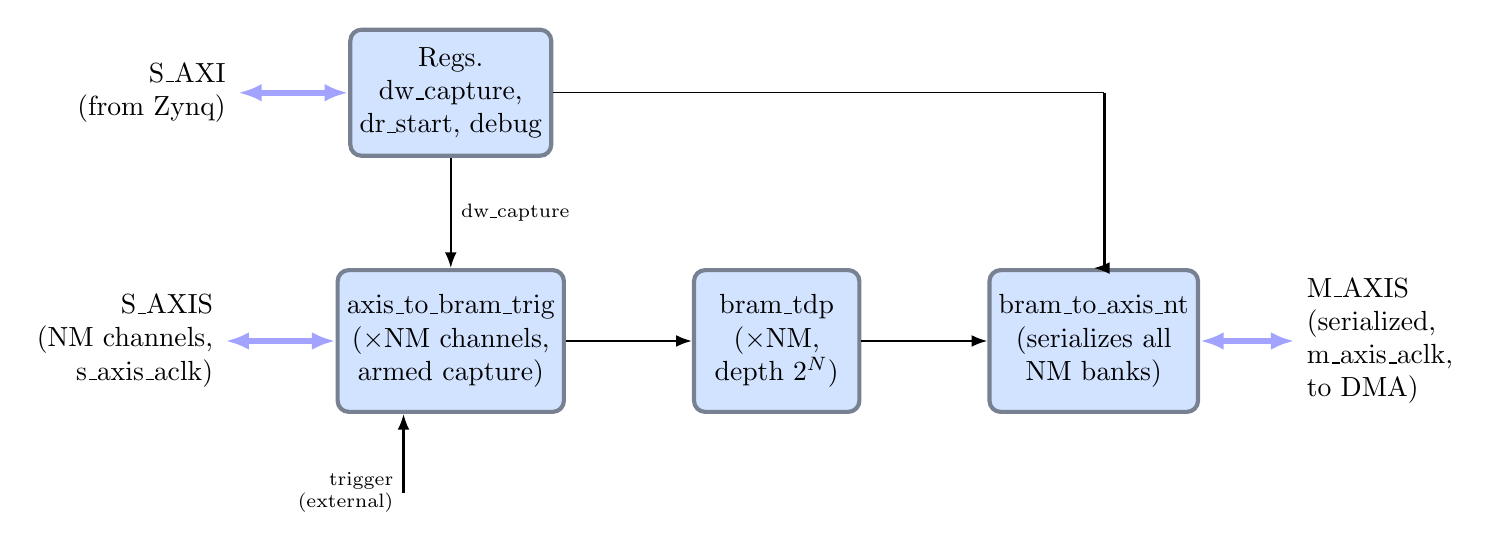
\begin{tikzpicture}
[box/.style={align=center, draw,rounded corners,minimum width=2.1cm,minimum height=1.2cm,draw={rgb,255:red,120; green,129; blue,145},fill={rgb,255:red,210; green,227; blue,255},line width=1.5pt},
arrow/.style={line width=2.2pt,draw={rgb,255:red,162; green,163; blue,255},{Latex[length=3mm]}-{Latex[length=3mm]}},
single arrow/.style={line width=0.8pt,-{Latex[length=2mm]}},
node distance=0.5cm]

% Regs.
\node[box,minimum height=1.6cm,minimum width=2.4cm] (regs) {Regs.\\dw\_capture,\\dr\_start, debug};

% Writer (armed capture, one per channel).
\node[box,below=1.4cm of regs,minimum height=1.8cm,minimum width=2.6cm] (writer) {axis\_to\_bram\_trig\\($\times$NM channels,\\ armed capture)};

% Per-channel BRAM.
\node[box,right=1.6cm of writer,minimum height=1.8cm] (bram) {bram\_tdp\\($\times$NM,\\ depth $2^N$)};

% Reader (serializes all NM banks on dr_start).
\node[box,right=1.6cm of bram,minimum height=1.8cm,minimum width=2.6cm] (reader) {bram\_to\_axis\_nt\\(serializes all\\ NM banks)};

% s_axi.
\draw[arrow] ($(regs.west)+(-1.4,0)$) node[anchor=east,align=right] {S\_AXI\\(from Zynq)} -- (regs.west);

% s_axis: write-side data (NM channels).
\draw[arrow] ($(writer.west)+(-1.4,0)$) node[anchor=east,align=right] {S\_AXIS\\(NM channels,\\ s\_axis\_aclk)} -- (writer.west);

% external trigger.
\coordinate (trig pin) at ($(writer.south)+(-0.6,0)$);
\draw[single arrow] ($(trig pin)+(0,-1)$) node[anchor=east,align=right,font=\scriptsize] {trigger\\(external)} -- (trig pin);

% regs -> writer (dw_capture arms it).
\draw[single arrow] (regs.south) -- (writer.north) node[pos=0.5,right,font=\scriptsize] {dw\_capture};

% regs -> reader (dr_start).
\coordinate (temp) at ($(regs.east)+(7.0,0)$);
	\draw[] (regs.east) -- (temp);
\draw[single arrow] (temp) |- (reader.north);

% writer -> bram.
\draw[single arrow] (writer.east) -- (bram.west);

% bram -> reader.
\draw[single arrow] (bram.east) -- (reader.west);

% m_axis.
\draw[arrow] (reader.east) -- ++(1.2,0) node[anchor=west,align=left] {M\_AXIS\\(serialized,\\ m\_axis\_aclk,\\ to DMA)};

\end{tikzpicture}

\end{document}
